%%%%%%%%%%%%%%%%%%%%%%%%%%%%%%%%%%%%%%%%%
% Structured General Purpose Assignment
% LaTeX Template
%
% This template has been downloaded from:
% http://www.latextemplates.com
%
% Original author:
% Ted Pavlic (http://www.tedpavlic.com)
%
% Note:
% The \lipsum[#] commands throughout this template generate dummy text
% to fill the template out. These commands should all be removed when 
% writing assignment content.
%
%%%%%%%%%%%%%%%%%%%%%%%%%%%%%%%%%%%%%%%%%

%----------------------------------------------------------------------------------------
%	PACKAGES AND OTHER DOCUMENT CONFIGURATIONS
%----------------------------------------------------------------------------------------
\documentclass{Askarticle}
\usepackage[utf8]{inputenc}
\usepackage{fancyhdr} % Required for custom headers
\usepackage{lastpage} % Required to determine the last page for the footer
\usepackage{extramarks} % Required for headers and footers
\usepackage{graphicx} % Required to insert images
\usepackage{lipsum} % Used for inserting dummy 'Lorem ipsum' text into the template
\usepackage{amsmath}
\usepackage{amsfonts}
\usepackage{listings}
\usepackage{color}
%\usepackage{slashbox}
\usepackage{verbatim}
\usepackage{graphicx}

\usepackage{fancybox}
\usepackage{tikz}

 \usepackage[utf8]{inputenc}
\usepackage[english]{babel}
 
\usepackage{amsthm}
 
\usepackage[colorinlistoftodos]{todonotes}
\usepackage{algorithm}
\usepackage{algpseudocode}

\usepackage{color} %for colored boxes
\usepackage{empheq}

\usepackage{listings} %to include Code

\usepackage{geometry}
 \geometry{
 a4paper,
 total={210mm,297mm},
 left=20mm,
 right=20mm,
 top=20mm,
 bottom=20mm,
 }

%---------------------------------------------------------------------------------------------
%LISTINGS INITIAL
%---------------------------------------------------------------------------------------------
\definecolor{codegreen}{rgb}{0,0.6,0}
\definecolor{codegray}{rgb}{0.5,0.5,0.5}
\definecolor{codepurple}{rgb}{0.58,0,0.82}
\definecolor{backcolour}{rgb}{0.95,0.95,0.92}
 
\lstdefinestyle{mystyle}{
    backgroundcolor=\color{backcolour},   
    commentstyle=\color{codegreen},
    keywordstyle=\color{magenta},
    numberstyle=\tiny\color{codegray},
    stringstyle=\color{codepurple},
    basicstyle={\ttfamily \footnotesize},
    breakatwhitespace=false,         
    breaklines=true,                 
    captionpos=b,                    
    keepspaces=true,                 
    numbers=left,                    
    numbersep=5pt,                  
    showspaces=false,                
    showstringspaces=false,
    showtabs=false,                  
    tabsize=2
}
 
\lstset{style=mystyle}
%---------------------------------------------------------------------------------------------
% Margins
\topmargin=-0.45in
\evensidemargin=0in
\oddsidemargin=0in
\textwidth=6.5in
\textheight=9.0in
\headsep=0.25in 

\linespread{1.1} % Line spacing

% Set up the header and footer
\pagestyle{fancy}
%\lhead{\hmwkAuthorName} % Top left header
\rhead{\hmwkClass\ : \hmwkTitle} % Top center header
%\chead{\firstxmark} % Top right header
\lfoot{\lastxmark} % Bottom left footer
\cfoot{} % Bottom center footer
\rfoot{Page\ \thepage\ of\ \pageref{LastPage}} % Bottom right footer
\renewcommand\headrulewidth{0.4pt} % Size of the header rule
\renewcommand\footrulewidth{0.4pt} % Size of the footer rule

\setlength\parindent{0pt} % Removes all indentation from paragraphs

%----------------------------------------------------------------------------------------
%	DOCUMENT STRUCTURE COMMANDS
%	Skip this unless you know what you're doing
%----------------------------------------------------------------------------------------

% Header and footer for when a page split occurs within a problem environment
\newcommand{\enterProblemHeader}[1]{
\nobreak\extramarks{#1}{#1 continued on next page\ldots}\nobreak
\nobreak\extramarks{#1 (continued)}{#1 continued on next page\ldots}\nobreak
}

% Header and footer for when a page split occurs between problem environments
\newcommand{\exitProblemHeader}[1]{
\nobreak\extramarks{#1 (continued)}{#1 continued on next page\ldots}\nobreak
\nobreak\extramarks{#1}{}\nobreak
}

\setcounter{secnumdepth}{0} % Removes default section numbers
\newcounter{homeworkProblemCounter} % Creates a counter to keep track of the number of problems

\newcommand{\homeworkProblemName}{}
\newenvironment{homeworkProblem}[1][Problem \arabic{homeworkProblemCounter}]{ % Makes a new environment called homeworkProblem which takes 1 argument (custom name) but the default is "Problem #"
\stepcounter{homeworkProblemCounter} % Increase counter for number of problems
\renewcommand{\homeworkProblemName}{#1} % Assign \homeworkProblemName the name of the problem
\section{\homeworkProblemName} % Make a section in the document with the custom problem count
\enterProblemHeader{\homeworkProblemName} % Header and footer within the environment
}{
\exitProblemHeader{\homeworkProblemName} % Header and footer after the environment
}

\newcommand{\problemAnswer}[1]{ % Defines the problem answer command with the content as the only argument
\noindent\framebox[\columnwidth][c]{\begin{minipage}{0.98\columnwidth}#1\end{minipage}} % Makes the box around the problem answer and puts the content inside
}

\newcommand{\homeworkSectionName}{}
\newenvironment{homeworkSection}[1]{ % New environment for sections within homework problems, takes 1 argument - the name of the section
\renewcommand{\homeworkSectionName}{#1} % Assign \homeworkSectionName to the name of the section from the environment argument
\subsection{\homeworkSectionName} % Make a subsection with the custom name of the subsection
\enterProblemHeader{\homeworkProblemName\ [\homeworkSectionName]} % Header and footer within the environment
}{
\enterProblemHeader{\homeworkProblemName} % Header and footer after the environment
}
   
%----------------------------------------------------------------------------------------
%	NAME AND CLASS SECTION
%----------------------------------------------------------------------------------------
\newcommand\given[1][]{\:#1\vert\:} %define new command
\newcommand{\hmwkTitle}{Homework\ \#1} % Assignment title
\newcommand{\hmwkDueDate}{\today} % Due date
\newcommand{\hmwkClass}{TIM\ 245 - Data Mining} % Course/class
\newcommand{\hmwkClassTime}{4:20pm} % Class/lecture time
\newcommand{\hmwkClassInstructor}{Instructor: Tyler Munger} % Teacher/lecturer
\newcommand{\hmwkAuthorNameB}{Panos Karagiannis}
\newcommand{\hmwkOption}{Homework Heavy Option}
\newcommand{\hmwkIDA}{ID: -}

\newcommand{\Prb}{\mathbb{P}}
\newcommand{\N}{\mathcal{N}}
\newcommand{\R}{\mathbb{R}}
\newcommand{\E}{\mathbb{E}}
\newcommand{\answer}{\noindent\rule{16cm}{0.9pt}
		
		\large{\textbf{\underline{Answer:}}}

		\vspace{0.5cm}}
%----------------------------------------------------------------------------------------
%	TITLE PAGE
%----------------------------------------------------------------------------------------

\title{
\vspace{2in}
\textmd{\textbf{\hmwkClass:\ \hmwkTitle}}\\
\normalsize\vspace{0.1in}\small{Due:\ \textit{\hmwkDueDate}}\\
\vspace{0.1in}\large{\textit{\hmwkClassInstructor}}
\vspace{3in}
}

\author{\begin{tabular}{ l r }
					 \hmwkAuthorNameB \\
					\multicolumn{1}{c}{\hmwkIDA}
				\end{tabular}}
\date{} % Insert date here if you want it to appear below your name

%----------------------------------------------------------------------------------------

\begin{document}

\maketitle

%----------------------------------------------------------------------------------------
%	TABLE OF CONTENTS
%----------------------------------------------------------------------------------------

%\setcounter{tocdepth}{1} % Uncomment this line if you don't want subsections listed in the ToC

\newpage
\tableofcontents
\newpage

\newtheorem{theorem}{Theorem}
\newtheorem{panostheorem}{Theorem}
\newtheorem{claim}[theorem]{Claim}
\newtheorem{definition}[panostheorem]{Definition}

%----------------------------------------------------------------------------------------
%	BLUE BOX
%----------------------------------------------------------------------------------------



\definecolor{myblue}{rgb}{.8, .8, 1}



\newlength\mytemplen
\newsavebox\mytempbox

\makeatletter
\newcommand\mybluebox{%
    \@ifnextchar[%]
       {\@mybluebox}%
       {\@mybluebox[0pt]}}

\def\@mybluebox[#1]{%
    \@ifnextchar[%]
       {\@@mybluebox[#1]}%
       {\@@mybluebox[#1][0pt]}}

\def\@@mybluebox[#1][#2]#3{
    \sbox\mytempbox{#3}%
    \mytemplen\ht\mytempbox
    \advance\mytemplen #1\relax
    \ht\mytempbox\mytemplen
    \mytemplen\dp\mytempbox
    \advance\mytemplen #2\relax
    \dp\mytempbox\mytemplen
    \colorbox{myblue}{\hspace{1em}\usebox{\mytempbox}\hspace{1em}}}

\makeatother

%----------------------------------------------------------------------------------------
%	PROBLEM 1
%----------------------------------------------------------------------------------------

\begin{homeworkProblem}[Problem \arabic{homeworkProblemCounter}: Exploratory Data Analysis in Excel ]
Open the csv dataset in Excel and identify 2-3 numerical attributes that you think would be potentially be good predictors  if a movie will receive an academy award. Then answer the following questions:

\begin{enumerate}
\item Provide a brief (1-2 sentence) explanation of each selected attribute and the rationale of why you think it would be a good predictor.
\item Use a combination of visual and quantitative tools to answer the following questions for each selected attribute:
\begin{enumerate}
\item	What is the typical value (central tendency)?
\item What is the uncertainty (spread) for a typical value?
\item What is a good distributional fit for the data (symmetric, skewed, long-tailed)?
\item	Does the attribute affect other attributes (correlation)?
\item	Does the attribute contain outliers (extreme values)?

\end{enumerate}

\end{enumerate}


It may be useful to format the answers as a table. Include any relevant plots and descriptive statistics in an appendix section.


\noindent\rule{16cm}{0.9pt}
		
\large{\textbf{\underline{Answer:}}}

\begin{enumerate}

\item After looking at the \textit{imdb} dataset the $3$ numerical attributes that I think could potentially be good predictors are:
\begin{enumerate}
\item \texttt{movie\_facebook\_likes} (column AA): \\The number of ``likes'' that a particular movie has gathered is a good indication of whether the movie has a strong public appeal. Therefore, we could assume that a large number of ``likes'' is evidence of the good quality of a movie.
\item \texttt{imdb\_score} (column Y):\\ Similarly to the number of ``likes'', the \texttt{imdb\_score} could function as a measure of the quality of a movie. Moreover, the \texttt{imdb\_score} is calculated using various filters and a weighted vote average rather than raw data averages (source: imdb website), Therefore, this measure could be even more reliable than the number of Facebook ``likes''.
\item \texttt{budget} (column V): \\ The budget of a movie could implicitly inform us about the quality of actors, directors and equipment used. These factors play an important role in the overall quality of a movie.
\end{enumerate}

%second question
 For each of the attributed chosen in part $(1)$ follow the answers to question $2$:\\

\texttt{movie\_facebook\_likes}: 
\begin{enumerate}
\item \textsc{Typical Value}: Calculating the mean for this data using Excel we get that the average number of ``likes'' is $7527$
\item \textsc{Spread}: The standard deviation (sample) for this data is $19,362$. Since significant outliers exist in this attribute a better measure of dispersion is $mad=163$
\item \textsc{ Distributional fit}: Drawing a histogram of the data we see that the distribution looks skewed to the right (i.e. few movies have a lot of likes)
\item  \textsc{Correlation}: In calculating the Pearson coefficient between  \texttt{movie\_facebook\_likes} and every other numerical attribute of this dataset we see that it is mostly positively correlated with  \texttt{num\_voted\_users} with correlation coefficient $\sigma=0.5397$, whereas, it is not negatively corelated with any other attribute.
\item 	\textsc{Outliers}: There exist many outliers which is evident from the magnitude of the measures of dispersion ($sd=19362$, $mad=163$).
\end{enumerate}

\texttt{imdb\_score}: 
\begin{enumerate}
\item \textsc{Typical Value}: Calculating the mean for this data and ignoring incomplete entries we get that the average score is approximately $6.43$
\item \textsc{Spread}: The standard deviation (sample) for this data is $1.117$
\item \textsc{distributional fit}: Drawing a histogram of the data we see that the distribution looks to be symmetric centered around the mean. 
\item  \textsc{Correlation}: In calculating the Pearson coefficient between \texttt{imdb\_score} and every other numerical attribute of this dataset we see that this attribute is not strongly correlated with any other attribute. \texttt{imdb\_score} exhibits the strongest positive correlation with \texttt{num\_voted\_users} ($\sigma=0.42$) and the strongest negative correlation with \texttt{facenumber\_in\_poster} ($\sigma=-0.06$). 
\item \textsc{Outliers}: Looking at the histogram as well as at the standard deviation ($sd=1.117$) there does not seem to be significant outliers for this attribute. Here we don't need to look at the $mad$ measure since our data are relatively symmetric around the mean.
\end{enumerate}

\texttt{budget}: 
\begin{enumerate}
\item \textsc{Typical Value}: Calculating the mean for this data and ignoring incomplete entries we get that the average budget is approximately $39,809,665.9916$
\item \textsc{Spread}: The standard deviation (sample) for this data is $206,468,209.615$. Since significant outliers exist in this attribute a better measure of dispersion is $mad=16,000,000$.
\item \textsc{Distributional fit}: Drawing a histogram of the data we see that the distribution looks to be similar to the number of Facebook likes, therefore it is very skewed to the right. 
\item  \textsc{Correlation}: In calculating the Pearson coefficient between \texttt{imdb\_score} and every other numerical attribute of this dataset we see that this attribute is not strongly correlated with any other attribute. \texttt{budget} exhibits the strongest positive correlation with \texttt{num\_critic\_review} ($\sigma=0.119$) and the strongest negative correlation with \texttt{facenumber\_in\_poster} ($\sigma=-0.01$). 
\item \textsc{Outliers}: Looking at the histogram as well as at the standard deviation ($sd=206468209$) and the median absolute deviation ($mad=16000000$) there seem to be significant outliers for this attribute.
\end{enumerate}

\end{enumerate}

$\implies$ \textsc{All histograms are included in the Appendix.}
\end{homeworkProblem}
% To have just one problem per page, simply put a \clearpage after each problem
%----------------------------------------------------------------------------------------
%	PROBLEM 2
%----------------------------------------------------------------------------------------

\begin{homeworkProblem}[Problem \arabic{homeworkProblemCounter}: Data Cleaning in Open-Refine]
\begin{enumerate}
\item Does the dataset contain missing values? What approach do you recommend for handling missing values?
\item What attribute, or combination of attributes, can be used as a unique identifier? Does the dataset contain duplicates?
\item Does the dataset contain outliers? What approach do you recommend for handling outliers?
\item Compare and contrast the following clustering methods. For each method provide examples from the IMDB dataset of where the method correctly identifies inconsistencies and where the method does not work.
\begin{enumerate}
\item	Key Collision / Fingerprint
\item	Nearest Neighbor / Levenshtein Distance
\end{enumerate}

\end{enumerate}
	
\noindent\rule{16cm}{0.9pt}
		
\large{\textbf{\underline{Answer:}}}

\begin{enumerate}
\item By looking at the entries for the selected attributes we realize that there exist many missing values. There are many different approaches that we could follow to handle such values, but in this case we can just ignore them because our data set is large, therefore we are discarding only a small fraction of data. For example, using OpenRefine we see that the number of entries whose budget is missing is only $434$ which is approximately $8\%$ of the total data. Similarly the fraction of missing imdb scores and facebook likes is $0.1\%$ and $0.02\%$, respectively.

\item First we check to see if the combination of attributes \texttt{movie\_facebook\_likes} and \texttt{imdb\_score} and \texttt{budget} can function as a unique identifier but unfortunately we see that there exist in total $462$ entries having all $3$ attributes common. Therefore we check to see whether the movie title is unique among all movies, nevertheless, it turns out that our dataset contains $117$ movie title duplicates. Therefore, we first remove the duplicate values of our attributes and then use as a unique identifier the combination of attributes \texttt{movie\_title} and \texttt{movie\_facebook\_likes}. \\

The number of total duplicate rows in the dataset is $40$. Since this is a small number of duplicates we can just remove them while only keeping the duplicates that we encountered first.

\item Based on our analysis in Question 1, we know that there exist outliers especially in the attributes \texttt{movie\_facebook\_likes} and \texttt{budget}. Therefore for all $3$ of our attributes we define $Q_{0}=5\%$ quantile and $Q_{1}=95\%$ quantile and then take the attributes which fall inside these quantiles. Following these process we only keep the following values:

 \[  0 \leq \texttt{movie\_facebook\_likes} \leq 47,350 \]
  \[  4.6 \leq \texttt{imdb\_score} \leq 8 \]
    \[  1,165,000 \leq \texttt{budget} \leq 140,000,000 \]
    
\item First, after filtering (following steps 1-3) my new dataset consists of $2929$ total entries. In comparing the two methods on the \emph{filtered} IMDB dataset we notice that \textit{Nearest Neighbor / Levenshtein Distance} performs a bit better than the simpler \textit{Key Collisions/ Fingerprint} method. More precisely, by trying the \textit{Key Collisions/Fingerprint} on \texttt{content\_rating} we see that it clusters together categories like \texttt{ \{ PG-13, PG\_13, pg13\} } nevertheless categories like \texttt{ \{ 13 pg, pg 13\} } are separately clustered. In those cases we had to intervene and make both categories clustered together. \\


Similarly, \textit{Nearest Neighbor / Levenshtein Distance} produced useful results for \texttt{content\_rating}. For example, this method created two seperate clusters for the ratings of \texttt{ \{Restricted, restricteed\} }, \texttt{ \{restricted, Restricted\} } where again we had to intervene and make both categories clustered together. Nevertheless, this method provided better results in other nominal values such as \texttt{movie\_title} and \texttt{director\_name}.
 
\end{enumerate}

 \end{homeworkProblem}


%----------------------------------------------------------------------------------------
%	PROBLEM 3
%----------------------------------------------------------------------------------------
\begin{homeworkProblem}[Problem \arabic{homeworkProblemCounter}: Data Integration and Transformation in Open-Refine]

\begin{enumerate}
\item Which normalization method did you use for your selected numerical attributes: min-max or z-score? Explain the reason for your selection.
\item	Examine one of the Wikidata film entries from the IMDB dataset (e.g. \texttt{https://www.wikidata.org/wiki/Q103474}). What other attributes in the Wikidata knowledge base could potentially be useful in predicting if a movie will win an academy award? 
\end{enumerate}

\textbf{Extra credit:}\\
Add the additional the attributes from your answer above to the IMDB dataset.

\noindent\rule{16cm}{0.9pt}
		
\large{\textbf{\underline{Answer:}}}
\begin{enumerate}
\item To normalize my data I chose the z-score normalization. In computing the z-score normalization I found it useful to recompute the mean and standard deviation of reach attribute since the removal of the outliers \emph{(Problem 2 Step 3)} reduced dramatically the standard deviation. The reason why I chose to use the z-score normalization is because it is more robust to outliers. Even if I have filtered the most significant outliers of my dataset for the selected attributes, there still exist outliers that could affect the linear normalization method of min-max.

\item In reviewing the Wikidata film entries from the IMDB dataset we see that the \texttt{based on} attribute could be useful in predicting if a movie will win an academy award. For example, if a movie is based on an award-winning novel then the chances of people and critics liking that movie are much higher. Moreover, another attribute that could allow us to make more accurate predictions could be the \texttt{depicts} attribute. For example, it could be the case that the majority of films that win academy awards depict ``space exploration'' or ``artificial intelligence'' therefore such information would be very insightful. 
\end{enumerate}
\end{homeworkProblem}
%----------------------------------------------------------------------------------------
%	PROBLEM 4
%----------------------------------------------------------------------------------------
\begin{homeworkProblem}[Problem \arabic{homeworkProblemCounter}: K-Nearest Neighbors Classification in Weka]
\begin{enumerate}
\item	What is the predictive accuracy of the kNN model? Do you think this model is good or bad? (We will cover model evaluation formally later in the quarter but I want to see how you think about model evaluation).

\item	What is the interpretation of the model, i.e. given the predictive accuracy what can we say about the relationship between the attributes and the target? For example, does the model support the hypothesis that the Academy Awards is a popularity contest?

\item	What are some of the applications of the predictive model? For example, who would be interested in this predictive model, e.g. directors, studios, actors, producers? How could they potentially use the model?

\item	What impact did the data cleaning from Problem 2 have on the predictive model? For example, what effect do missing values, duplicates, outliers, and inconsistencies have in the kNN model?

\item	What impact did the data transformation from Problem 3 have on the predictive model? For example, how does normalization affect the kNN model?

\item	What are some of the potential issues with the classification model? What are some possible improvements that could be made to address these issues?

\textbf{Extra credit:}\\
Implement the improvements your suggested improvements above and re-evaluate the model. Do the improvements make a difference in the model?s prediction accuracy? Explain why or why not?


\end{enumerate}



\noindent\rule{16cm}{0.9pt}
		
\large{\textbf{\underline{Answer:}}}

\begin{enumerate}
\item In our KNN classifier, we trained for parameter values $K=1$, using the Euclidean distance and testing using 10-fold cross validation. The accuracy of the classifiers is: 

\[ Accuracy= 90.4051\% \pm 5.1992\% \]

,where $90\%$ reflects the mean value among all 10 training samples and $5\%$ reflects their standard deviation. I believe that whether the model is good or bad depends on the specific application. For example this model is good if we want to utilize it as evidence that the Academy Awards are strongly dependent on these $3$ attributes. Nevertheless, if we were to use this model to bet a lot of money on a specific movie winning the Academy Award, then the precision is very low.

\item Based on our predictive accuracy it seems that our model is able to predict fairly accurately whether a movie will win the Academy Award based on these $3$ attributes. Since the attributes we used are \texttt{movie\_facebook\_likes}, \texttt{imdb\_score} and  \texttt{budget}, the model indeed verifies the hypothesis that the Academy Awards is a popularity contest.

\item A potential use of the model would be for producers to be able to sign contracts in advance with the actors/directors participating in the movie. After a movie has won the Academy Award then the popularity of the actors as well as the directors increases and therefore it would be harder and more expensive to sign contracts with them.

\item The cleaning of the data in Problem 2 was very significant. For example \emph{duplicate} values can alter the final results by introducing biases in our model. Moreover, since \emph{outliers} are extreme values that do not occur often, they make our classifier more inaccurate. Finally, we chose to discard the \emph{blank} values instead of, for example, assigning them the typical value of the attribute. Nevertheless, I believe that this choice is safer since we have a lot of data and also we don't know what the exact actual entries for each attributed were. 

\item Normalizing the values in Problem 3 had a very significant impact on the model. For instance, the imdb scores are in the range of $[0,10]$ whereas the budget range is of $[0, 10^{8}]$. Since we used the Euclidean distance in our model, the term differences of the budget would dominate the sum. As a result, the ``effect'' of the \texttt{imdb\_score} in our model would be diminished. 

\item A potential issue with this classification model is that we are using only three attributes to predict whether a movie is likely to win the Academy Award. Nevertheless, there are still many attributes that play a significant role and that could help us improve our accuracy. Moreover, there is no guarantee that the Euclidean Distance is the best similarity measure for our application. There is a variety of other similarity measures that we could use in our model such as the \emph{Manhattan Distance, Chebyshev Distance or the Minkowski Distance}. Moreover, in our model we chose the value of $K$ to be $1$. Nevertheless, the value of $K$ plays a significant role in the accuracy of our model, therefore we could experiment further with our model by increasing $K$.

\end{enumerate}

\textbf{Extra Credit}

Table 1 displays the accuracy of the model for all different similarity measures that were previously suggested. For consistency, the formulas for each of these methods are also included:
\[ D_{EUCL}(\vec{d_{1}},\vec{d_{2}})= \sqrt{ \sum_{i=1}^{m} \left[\vec{ d_{1}}(i)-\vec{d_{2}}(i) \right]^{2}} \]
\[ D_{MANH}(\vec{d_{1}},\vec{d_{2}})=  \sum_{i=1}^{m} \left| \vec{ d_{1}}(i)-\vec{d_{2}}(i) \right| \]
\[ D_{CHEB}(\vec{d_{1}},\vec{d_{2}})=  \max \left| \vec{ d_{1}}(i)-\vec{d_{2}}(i) \right| \]
\[ D_{MINK}(\vec{d_{1}},\vec{d_{2}},p)=  \sqrt[\leftroot{-2}\uproot{2} p]{ \sum_{i=1}^{m} \left[\vec{ d_{1}}(i)-\vec{d_{2}}(i) \right]^{p}} \]


\begin{table}[H]
		\caption{Accuracy for different similarity measures and $K=1$}
		\centering
		\begin{tabular}{c c c}
		\hline\hline
		$Method$ & Accuracy(\%) & Standard Deviation(\%) \\ [0.5ex] % inserts table %heading
		\hline
		Euclidean & 90.4051 & 5.1992 \\  
		Manhattan&90.0975 &4.5370 \\
		Chebyshev&90.2002 & 4.7263\\
		Minkowski (p=5) &90.0977& 4.7843 \\
		%\\ [1ex]
		\hline
		\end{tabular}\\[0.5cm]
		\label{table:nonlin}
\end{table}

Using the table we notice that the Euclidean Distance outperforms all the other Distances. As a result we take the Euclidian distance and we experiment with the different values of $K$, summarizing our results in Table $2$.

\begin{table}[H]
		\caption{Accuracy for different values of $K=1$ using the Euclidean Distance}
		\centering
		\begin{tabular}{c c c}
		\hline\hline
		$K$ & Accuracy(\%) & Standard Deviation(\%) \\ [0.5ex] % inserts table %heading
		\hline
		1 & 90.4051 & 5.1992 \\  
		10&93.9215 & 2.8447 \\
		20&94.3999 & 2.6574\\
		50 &94.2288& 2.8853 \\
		%\\ [1ex]
		\hline
		\end{tabular}\\[0.5cm]
		\label{table:nonlin}
\end{table}

We see that the best performance increases as we reach $K=20$ and then decreases as we further increase $K$ to reach $50$. As a result we notice that in order to produce more accurate predictions we need to increase the value of $K$ which implies that we are using more ``neighbors'' in order to classify a given movie. This is logical, in the sense that we are using more information to make a decision. Moreover, it is worth mentioning that the standard deviation decreases as we increase $K$ which means that we are now more certain about our classification. Nevertheless, we see that the as we increase the value of $K$ to reach $50$ the accuracy of our model starts decreasing. The reason for this is overfitting, which basically means that we are attempting to match too closely our training data while at the same time becoming less flexible in classifying our test data.
		
\end{homeworkProblem}



%----------------------------------------------------------------------------------------
%	Appendix
%----------------------------------------------------------------------------------------
\newpage
\begin{homeworkProblem}[Appendix]

\noindent\rule{16cm}{0.9pt}

\begin{figure}[htp]

\centering
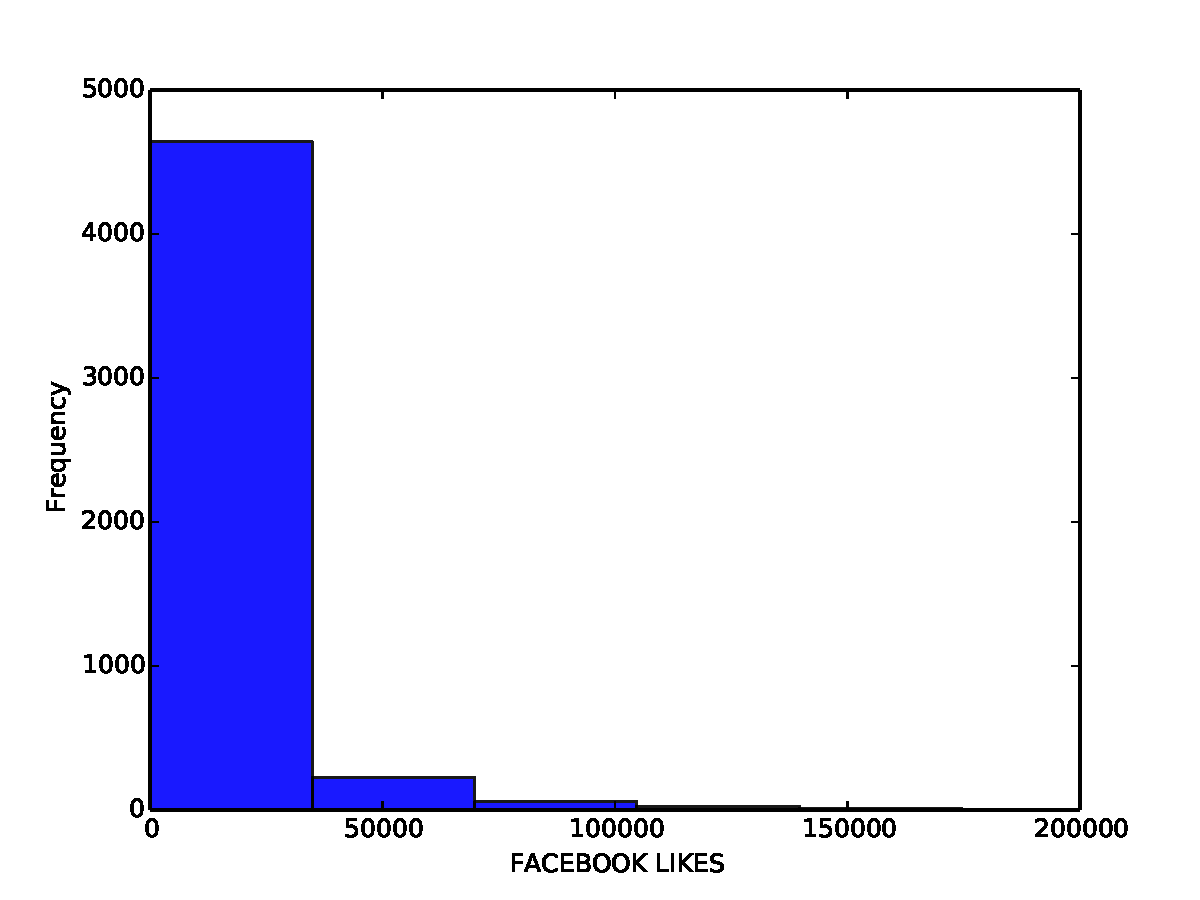
\includegraphics[width=.5\textwidth]{fb_hist.pdf}\hfill
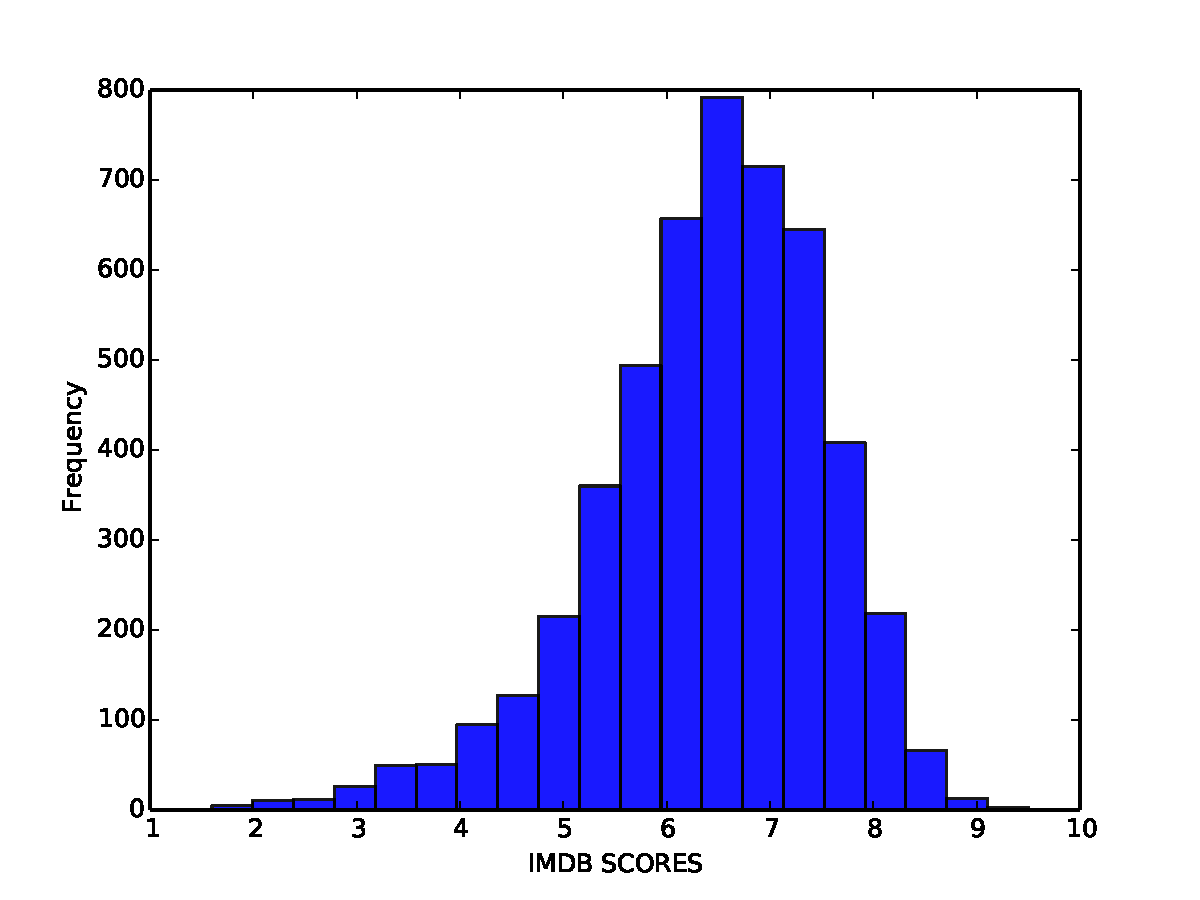
\includegraphics[width=.5\textwidth]{imdb_hist.pdf}\hfill
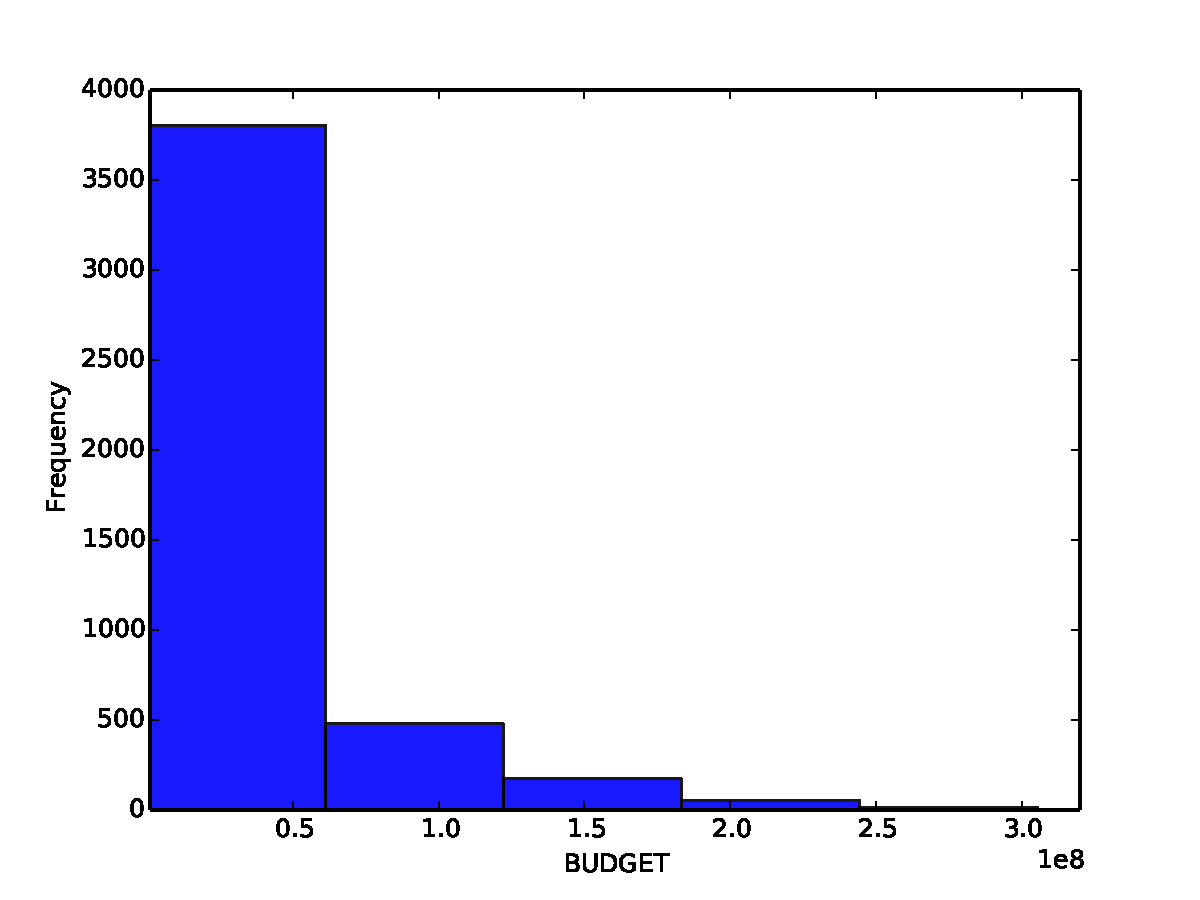
\includegraphics[width=.5\textwidth]{budget_hist.pdf}

\caption{Histograms for the $3$ selected attributes for Question 1}
\label{fig:figure3}

\end{figure}

\end{homeworkProblem}




\end{document}
